\documentclass{article}

% if you need to pass options to natbib, use, e.g.:
%     \PassOptionsToPackage{numbers, compress}{natbib}
% before loading neurips_2022


% ready for submission
%\usepackage[final]{neurips_2022}


% to compile a preprint version, e.g., for submission to arXiv, add add the
% [preprint] option:
%     \usepackage[preprint]{neurips_2022}


% to compile a camera-ready version, add the [final] option, e.g.:
%     \usepackage[final]{neurips_2022}


% to avoid loading the natbib package, add option nonatbib:
%    \usepackage[nonatbib]{neurips_2022}


\usepackage[utf8]{inputenc} % allow utf-8 input
\usepackage[T1]{fontenc}    % use 8-bit T1 fonts
\usepackage{hyperref}       % hyperlinks
\usepackage{url}            % simple URL typesetting
\usepackage{booktabs}       % professional-quality tables
\usepackage{amsfonts}       % blackboard math symbols
\usepackage{nicefrac}       % compact symbols for 1/2, etc.
\usepackage{microtype}      % microtypography
\usepackage{xcolor}         % colors
\usepackage{graphicx}


\title{Graph-Based Deep Learning for Fraud Detection in ETH Transaction Networks}


% The \author macro works with any number of authors. There are two commands
% used to separate the names and addresses of multiple authors: \And and \AND.
%
% Using \And between authors leaves it to LaTeX to determine where to break the
% lines. Using \AND forces a line break at that point. So, if LaTeX puts 3 of 4
% authors names on the first line, and the last on the second line, try using
% \AND instead of \And before the third author name.


\author{
  Gelinas, Stephen \\
  \texttt{sgelinas@ucsd.edu} \\
  \And
  Yamamoto, Kazuma \\
   \texttt{kayamamo@ucsd.edu} \\
  \And
  Zhou, Ethan \\
  \texttt{ezhou@uscd.edu} \\
}


\begin{document}


\maketitle

\begin{abstract}
 	Blockchain technology is a quickly growing field, helped greatly through its widespread applications in the financial field. However, the space has been under attack through phishing fraud, posing itself as a major threat to blockchain security. According to the FTC, cryptocurrency scams have cost online users over \$1 Billion since 2021; there is a clear demand for the development of effective fraud detection strategies to prevent and detect cybercrimes. With access to Ethereum transaction networks, we can model and train phishing detection as a node classification problem. With graph-based machine learning approaches, we can more effectively flag fraudulent activity in Ethereum networks and reduce the amount of phishing activity with Ethereum, and improve user experience with safer transactions as blockchain technology gains even more traction.
\end{abstract}


\section{Introduction}
    Blockchain technology allows for the process of recording transactions and tracking assets between two parties without a third party. Recently, many applications have been using blockchain technology, exchanging cryptocurrency such as Bitcoin and Ethereum. However, the amount of phishing scams, money laundering, and other cybercrimes have risen within these blockchain platforms. These crimes are difficult to investigate and identify the offender due to the high frequency of transactions. Traditionally, banks are utilized as the third party or intermediary to constantly monitor and check when a new account is opened or suspicious transactions are made. However, in our case with blockchain, people are easily able to create wallets and make transactions freely, thus creating the concern that it may be difficult to check for suspicious or crime-related transactions. Due to the nature of blockchain technology, transaction information is held public and anyone can attain this information, but this may not be sufficient to detect suspicious activity. As blockchain and cryptocurrency becomes more popular, the number of transactions and wallets increase also, causing detection of suspicious transactions to be more difficult and time-consuming.  
    
	Due to the potential cybercrimes that may occur from blockchain, many studies have been conducted to detect suspicious transactions in expansive financial networks. Some of these studies have utilized timestamps, incidental expenses, or the number of transactions as their features for their models. In addition, some studies have also utilized graph embeddings for model optimization and evaluation of fraud detection. However, there are only a few studies out that have been conducted using graph neural network (GNN) models. Recently, a deep learning approach graph convolution algorithm has been popularized to automatically generate features using nodes and edges of graphs. The Graph Convolutional Model (GCN) applies neural network models to graph data, and it learns by updating feature values of each node and edge based on the graph structure. 


In our study, we will use public Ethereum transaction networks as our graph data, and we will examine GNN in comparison to multiple other traditional models to determine the most effective method in detecting phishing fraud transactions. To achieve this, a graph is first constructed from the Ethereum transaction data, then we incorporate graph models such as GCN, GraphSage, and Graph Attention Network (GAT). The performance of these models is then compared to traditional models such as XGBoost, K-Nearest Neighbors (KNN), and Support Vector Machines (SVM). Our source code is available here. 
	
\begin{center}
\url{https://github.com/KazumaYamamoto2023/DSC180B-Q2-Project}
\end{center}


\section{Methods}

\subsection{SVM}
    Our group started off with a support vector machine model (SVM) to act as our first non-graph model. This is a supervised machine learning algorithm with the objective to find the most optimal hyperplane that can best separate data points of different classes in an N-dimensional space (N being the \# of features). Each transaction is represented as a vector, with each feature of the transaction (sent\_eth, received\_eth, pagerank) as a dimension in space. It then identifies the features that are most important for separating fraudulent and non-fraudulent transactions and finds the hyperplane that best separates the two classes. Because this is a supervised learning approach, we filtered out the unlabelled data and achieved an accuracy of $\sim$$60.5\%$ with this classification model. 


\subsection{KNN}
        Our second non-graph approach is a K-Nearest Neighbors model, where the features of each transaction are utilized to create a feature vector. The distance is then calculated between each feature vector of the test set and the existing feature vectors of the training set. The nearest transactions based on the smallest distances are identified and its label (fraudulent or non-fraudulent) is determined by its neighbors. For this algorithm, we achieved an average accuracy of $\sim$$74.6\%$, which is higher than our first baseline using SVM. 

\subsection{XGBoost}
        For our last non-graph approach, we decided to use XGBoost (Extreme Gradient Boosting), which is an ensemble method that combines weak decision trees to create a stronger predictive model (boosting technique). This algorithm works by iteratively building decision trees and adjusting the weights of the transaction edges to minimize loss. XGBoost obtained an average accuracy of $\sim$$81.6\%$, which is higher than some of the traditional and graph models we implemented. 


\subsection{Node2Vec}
	Node2vec as an algorithm solves the problem of transforming the information inherent within a network into a workable numeric representation by transforming each node into a vector. The first step in this process is done through a random walk algorithm. In our case, the edges between the nodes are given weights corresponding to the transaction amount between accounts. These weights are used to simulate random paths between nodes from the network. In the next step, the skip-gram model works with these paths to learn and creates a node embedding for each node. How this is done is that it reads the random paths taken, and learns which nodes are likely to precede another node. These embeddings then allow us to determine the makings of a fraudulent account. We achieved the best results through the pytorch implementation, with roughly a $\sim$$76.6\%$  accuracy on the test set. The pytorch package allows us to make use of the large amount of unsupervised nodes present in our dataset, improving performance.


\subsection{GraphSage}

	GraphSage is most known for its inductive nature which allows it to better adapt to previously unseen nodes. In a setting like Ethereum transaction networks where the network evolves with new nodes and edges every day, there would be a benefit to using a model that does not have to be retrained every time new information is introduced. Additionally, in comparison to methods like node2vec, GraphSage has the advantage of being able to learn from node features. GraphSage works by starting at a node and aggregating information on its neighbors to generate the embeddings. The pytorch package for this model produced an accuracy of $\sim$$81.9\%$, a noticeable upgrade compared to node2vec. This difference can be attributed to the fact that in a largely unsupervised dataset, an inductive approach may outperform the deductive approach.


\subsection{GCN}
	We worked with GCNs in our first quarter on our Clickbait Detection algorithm with TextGCN and we have implemented a version for this task as well. Much of the structure is the same; we create an adjacency matrix based on the edges of the network then propagate steps forwards (3 in our case) then form node embeddings based on these. From there, we can iterate through the nodes and update the node features by hashing the features of each neighboring node. The GCN model from pytorch produced an accuracy of $\sim$$79.6\%$.

\subsection{Graph Attention Network}
	We also tested the performance of Graph Attention Networks (GAT). GATs are a type of graph neural network that leverages masked self-attention which addresses the shortcomings of prior methods based on graph convolutions or their approximations. With GATs, we are able to extract meaningful node features by implicitly specifying different weights got different nodes in a neighborhood, without requiring costly matrix operations nor knowing the underlying graph structure upfront. GAT outperformed GCN and GraphSAGE on node classification tasks on the Cora dataset, so we hypothesized that this model may have similar performance on our dataset compared to other models. The GAT model from pytorch produced an accuracy of $\sim$$78.5\%$, and slightly underperformed compared to GCN and GraphSAGE.

\subsection{Adaptive - GCN}
	The final model we evaluated was Topology Adaptive GCN (TA-GCN). TA-GCN is a graph neural network defined in the vertex domain and outperforms many spectral graph convolutional neural networks (CNNs). TA-GCN utilizes a set of fixed-size learnable filters to perform convolutions on graphs. The topologies of these filters are adaptive to the graph’s topology when scanned for convolutions. TA-GCN inherits the properties of convolutions in CNNs for grid structured data, yet doesn’t require approximation to compute the convolution, leading to greater performance relative to spectral CNNs. TA-GCN is also computationally simpler than other graph neural networks. Additionally TA-GCN tends to achieve comparable or better accuracy than GCN and GraphSAGE for datasets with larger and sparser graph structures. We hypothesized that the sparsity of our transaction network will be beneficial for TA-GCNs performance in our node classification prediction task. We implemented a TA-GCN model using pytorch, which produced an accuracy of $\sim$$82.2\%$, outperforming all of our models for comparison.
 
\section{Results}
    We conducted a comparative model performance evaluation experiment using graph and non-graph models to detect phishing fraud accounts against an Ethereum transaction network. Graph-based features improve overall model performance for both graph-based and non-graph-based models. Graph neural networks, specifically TA-GCN, performed best in the fraud detection task, as GNNs are able to learn the networks’ structural information. 

    Model performance was determined by taking the average classification accuracy on the testing set over 10 model runs. The resulting classifier performance for this prediction task are shown in Table 1:
    
\begin{table}[h]
\centering
\begin{tabular}{ |c|c|c| } 
	\hline
	Model & Avg. Testing Accuracy & Type \\
	\hline \hline
	TA-GCN & 82.2 & Graph \\ 
	\hline
    GraphSage & 81.9 & Graph \\ 
	\hline
	XGBoost & 81.6 & Tree \\ 
	\hline
	GCN & 79.6 & Graph \\ 
	\hline
	GAT & 78.5 & Graph \\ 
	\hline
	Node2Vec & 76.6 & Graph \\ 
	\hline
	k-NN & 74.6 & Traditional \\ 
	\hline
	SVM & 60.5 & Traditional \\ 
	\hline
\end{tabular}
\caption{Performance of each model}
\end{table}

    The most important features for predicting fraudulent wallets are pagerank and the maximum amount of ETH sent between wallets as shown in Figure 1.

\begin{figure}[h]
	\centering
	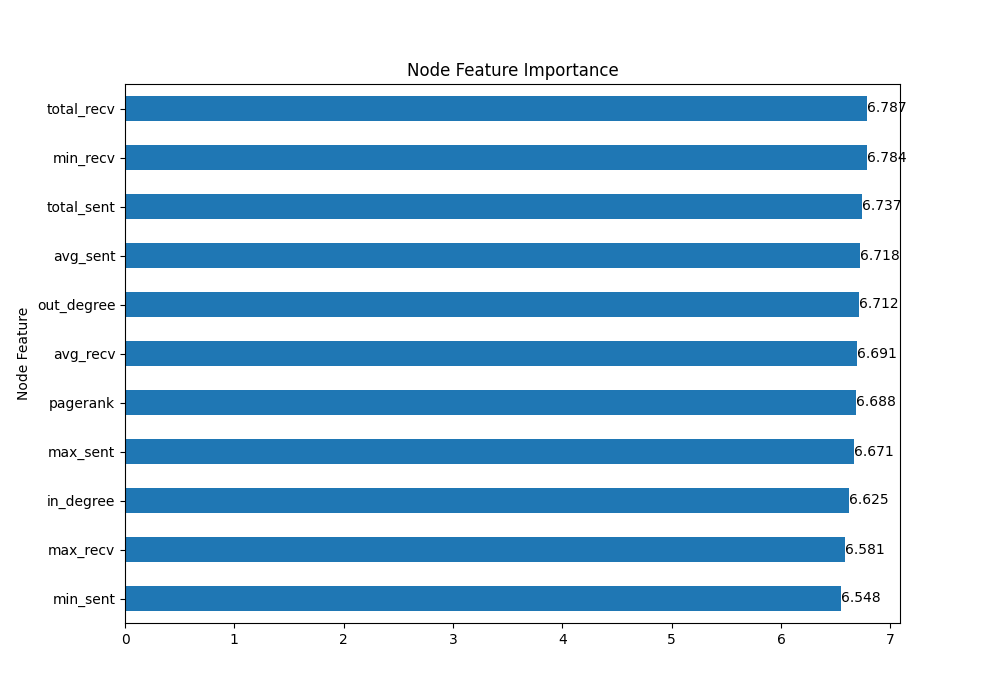
\includegraphics[width=0.8\linewidth]{images/tagcn_feat_imp.png}
	\caption{The relative importance of each feature to our models}
\end{figure}
    
\section{Discussion}
    From our results, we found that the effectiveness of these algorithms depend on the models being used. For instance, we formed a hypothesis on why TA-GCN performed the best. The graph convolution of TA-GCN is characterized by multiplying polynomials of the graph adjacency matrix without any involved approximations, while traditional GCN models are based on approximating the convolution. Our performance improvements stem from the fact that we accurately capture the underlying graph structure without approximations during the convolution operation. In addition, filter topology is adaptive to the topology of the graph when scanning the graph to perform convolution, which allows for a better understanding and learning of the graph structure. This is in contrast to traditional GCN, which relies on fixed filters. Lastly, TA-GCN is computationally simpler and exhibits better performance when dealing with less sparse graphs. Given that our transaction network is not particularly sparse, this suggests that TA-GCN is well-suited for our network and may perform particularly well. 

    In addition, our hypothesis regarding why XGBoost performed better than some GNNs is based on several factors. Firstly, XGBoost has the ability to learn from unlabelled data, taking advantage of all the training data similar to the GNN models we chose, thus improving predictive power. Additionally, XGBoost includes an early stopping feature that can help lessen the risk of overfitting, by stopping the training process once the model’s performance begins to worsen. However, XGBoost tends to perform worse when dealing with sparse data and imbalanced data. Fortunately, our transaction network is not sparse and our training set is not imbalanced, which means that XGBoost is not at a disadvantage in these regards. 

    Lastly, GNN models performed better than traditional models due to their ability to utilize the full training set of unlabelled data. KNN and SVM, for example, require all labeled data or nodes for training, which can limit their effectiveness. GNNs, on the other hand, are able to leverage both labeled and unlabeled data, improving their ability to learn from the full training set.
    

\section{Conclusion}
    From our experiment, we found that graph networks are a more powerful tool for modeling complex relationships in comparison to traditional non-graph models. Evaluating and improving machine learning models can have a significant impact on the accuracy and efficiency of fraud detection. Better models can detect more subtle patterns of fraudulent activity or reduce false positive rates, where real transactions are incorrectly flagged as fraudulent, improving the overall effectiveness to correctly detect fraudulent behavior. Improving these graph models can offer advantages such as minimizing financial losses for people using Ethereum and developing trust in the Ethereum ecosystem. Furthermore, since Ethereum is a constantly growing platform, it’s essential to constantly evaluate and update machine learning models to prevent new types of fraud and adapt to changes in blockchain, ensuring the security and integrity of Ethereum. For future work, we may explore other types of algorithms that require different data structures and perhaps combine existing models to develop a model for specific tasks in blockchain. 


\section{Appendix}
	Blockchain technology has been growing in use through its widespread applications in the financial field. However, it has recently attracted increasing cybercrimes with phishing fraud emerging as a major threat to blockchain security. With graph-based machine learning approaches, we can more effectively flag fraudulent activity in Ethereum networks, to reduce the amount of phishing activity with Ethereum, and increase user trust with safe transactions as blockchain technology gains widespread adoption. This problem is similar to our Quarter 1 project in that we are attempting to classify nodes from a network of nodes and edges. However, in Quarter 1 our project required text to be present in the data since we were using TextGCN to classify the nodes. This quarter, our project will not require any text and will rely more heavily on the weights on the edges between nodes in the form of transaction amount. We aim to achieve a high accuracy while working with less information per node-edge than before. There have been some similar analyses in the past, most notably by one of our mentors, Parker Erickson, who has done some analyses into fraud detection using TigerGraph with Graph Attention Networks. However, we propose that we use a richer selection of models and pull more meaningful features from our dataset. We extracted additional node features using GSQL queries by utilizing our dataset’s multigraph structure. We computed features of in-degree and out-degree, weighted by the total number of transactions between nodes. Additionally, we computed additional summary statistics such as the sum, mean, minimum and maximum amount of Ethereum sent and received between addresses. We also chose to evaluate the performance of four additional models: Graph Convolution Networks, Node2Vec, GraphSAGE, and Topology Adaptive Graph Convolution Networks. We believe this richer selection of models will lead to better performance in our prediction task, relative to that of Graph Attention Networks, due to the sparsity of our transaction graph’s structure. We will evaluate each model by taking the mean testing accuracy in 10 model runs. Our primary output will be a website. Our paper will be successful because we already have access to a dataset with the exact information we need. The dataset contains nodes of accounts and edges of transactions, which is what we are looking for to run node classification.


\end{document}